\chapter{Deta analysis}
\label{chapter:analysis}
The HADES experiment has performed a proton-proton experiment with protons kinetic energy 3.5 GeV in September 2018. Data collected during this experperiment allowed to conduct a series of analysis devoted to hypererons studies \cite{hades_inclL_35,hades_L1405,hades_L1520,hades_PWA_pKpL,hades_S1385}. In the following thesis the next step of hyperon studies is presented. The four particles $\p \pim \pip \pim$ final state was analyzed. Is allows to reconstruct the inclusive signals of a $\Ls$ and  a $\Lz \Kz$ production. The obtained results were compared with previous, exclusive measurements and used to constrain simulation of a new esperiment devoted to hyperon studies \ref{chapter:simulations}.

All methodes developed for pp@3.5 GeV experiment were also used for deta deriving from pNb@3.5GeV experiment. In result an inclusive \cs for $\Ls$ together with the reference state $\Lz \Kz$ were measured. Compare to previous HADES studies \cite{hades_Sz_pNb,hades_Lp_femtoscopy_pNb,hades_arnold_pNb,hades_Ksi_pNb} it allows to extend knowladge about hyperons in pNb reactions  Additionaly to obtain a background description an event mixing metode was used.

\section{Paricles identyfication}
The HADES detector allows for two complementary methodes of particles analysis. The first, bases on particles' time of flight measured in the ToF detectors and particle's momentum measured in the MDC. The second methode, bases on the MDC exclusively and uses combide information about particles' momentum and energy losses. The first one is favoured due to better precision, however a limited geometrical acceptance of the TOF detectors reduces detection efficiency by a factor 0.8 for each particle. In case of four particles final state, discussed in this thesis, a total loss caused by the TOF detectors  can reach 60\% of all detected particles. For that reason the $\frac{de}{dx}$ vs. $\p$ identyfication metode was used. The identyfication cuts were opimized for previous analysis conducted by by HADES experiment and described in \cite{hades_inclL_35,lalik_phd}. Contours used for $\pim$ and $\pip$ are the same and differes only by electric charge.

\section{Event selection}
Among all registered events only these containing at least four charged particles (two positive and two negative) was considered in analysis. They were observed events with more than four particles detected. They produces kombinatorics which are very difficould to controll during further analysis. Becouse of that only one four-particle combination from every event was taken. The combinations were ordered according to track reconstruction quality and the best one was choosen. 
\section{Reaction kinematics}
\label{section:kinematics}
For pp@3.5 GeV collisions the production threshold for $\Ls$ ($E^{\mathrm{thr}}_{\p\Kp\Lz}=$) lies just below avaliable energy ($\Sqs=$). Using the rule of a energy-momentum conservation is possible to calculate missing mass for observed particles. Because the analized final state is produced via reaction
\begin{equation}
  \p\p \rightarrow \p \Kp \Ls [\Lz \pip \pim],
\end{equation}
the smallest missing mass for the signal channel is $\Sqs - \Ls_{mass}= 1432$ MeV. It is a very strong kinematical constrain wich seperates well the signal from most of background channels. The missing mass spectrum is presented in fi.g \ref{fig:missMass}. There is visible a resonanse behavour around 1200 MeV. Due to a charge conservation rule missing particles have to have a total charge +2. It leeds to the conclusion that the missing mass spectrum is dominated by a $\Dpp$ production.

\begin{figure}[hb]
  \centering
  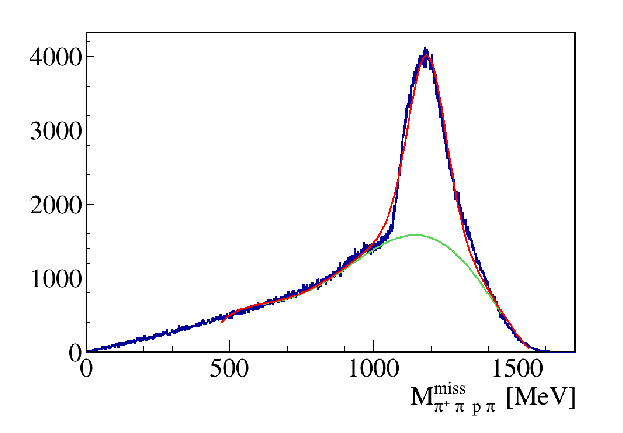
\includegraphics[width=0.9 \linewidth]{Chapter_analysis/missMass.eps}
  \caption{The missing mass of $\p \pim \pip \pim$ system. The resonance behavour around 1200 MeV is cleary visible. The read line represents sum of signal (a Voigt function) and a background (5-th order polynomial) fit. Fited Voigt function gives following parameters: $\bar{M}=1186$ MeV, $\sigma=61$ MeV, $\Gamma=$20 MeV.}
  \label{fig:missMass}
\end{figure}


Because in HADES energy regime almost all pions are produced via barionic resonances, and $\Dpp$s tend to be produced in pairs, it was expected that an invariant mass of $\p \pip$ detected in experiment would also contain a $\Dpp$ component. Indeed, as it is shownn in fig. \ref{fig:dpp2D} most of the background comes from coreleted source with mass maximum around double $\Dpp$ production. The figure shows also that a cut on missing mass > 1432 MeV remuves a significant part of a background events. In case of $\Lz \Kz$ channel (see. \ref{section:LzKz}) the missing mass cut was put on a lower mass ??.

\begin{figure}[hb]
  \centering
  %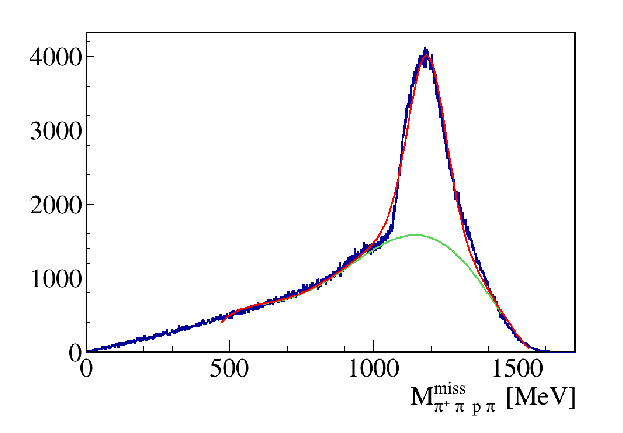
\includegraphics[width=0.9 \linewidth]{Chapter_analysis/missMass.eps}
  \caption{The missing mass of $\p \pim \pip \pim$ system vs. invariant mass of a $\p\pim$ system. It is creary visible that most of the bacground comes from corelated source of two $\Dpp$ production. Such situation helps to easy discriminate most of the background.}
  \label{fig:dpp2D}
\end{figure}

\section{The $\Lz$ Reconstruction}
The next step of the analysis after a missing mass cut was an inclusive $\Lz$ reconstruction. In previous HADES experiments the reconstruction had based on a set of geometrical cuts. Their role was to increase signal-to-background ratio utlizing a $Lz$ decay gemetry. Because the $\Lz$ decasys via week interactions its livetime is relatively long:$c\tau = 7.89 cm$ \cite{PDG}. That may be used to discriminate an out of target vertex from a background originates from a target.

As it was shown in \ref{section:kinematics} an avaliable phase-space for $\Ls$ production for a $E_k=3.5$ GeV is very limited. An inlusive analysis performed in \cite{hades_L1520} has measured ?? events of $Ls$ after all cuts. To impruve statistics, and also axminate new reconstruction methodes in following analysis a neural network was used as a replacement of the geometrical cuts. Details about used methode are explaned in chapter \ref{chapter:NN}.

The opitimalized neural network enhanced a signal to bacgkround ratio from ??? without any cuts to ???. A $\Lz$ signal obtained in this way was used for a next steps of analysis: the $\Ls$ analysis (chapter \ref{section:Ls}) and asocieted $\Lz \Kz$ production (chapter \ref{section:LzKz});

\begin{figure}[ht]
  \centering
  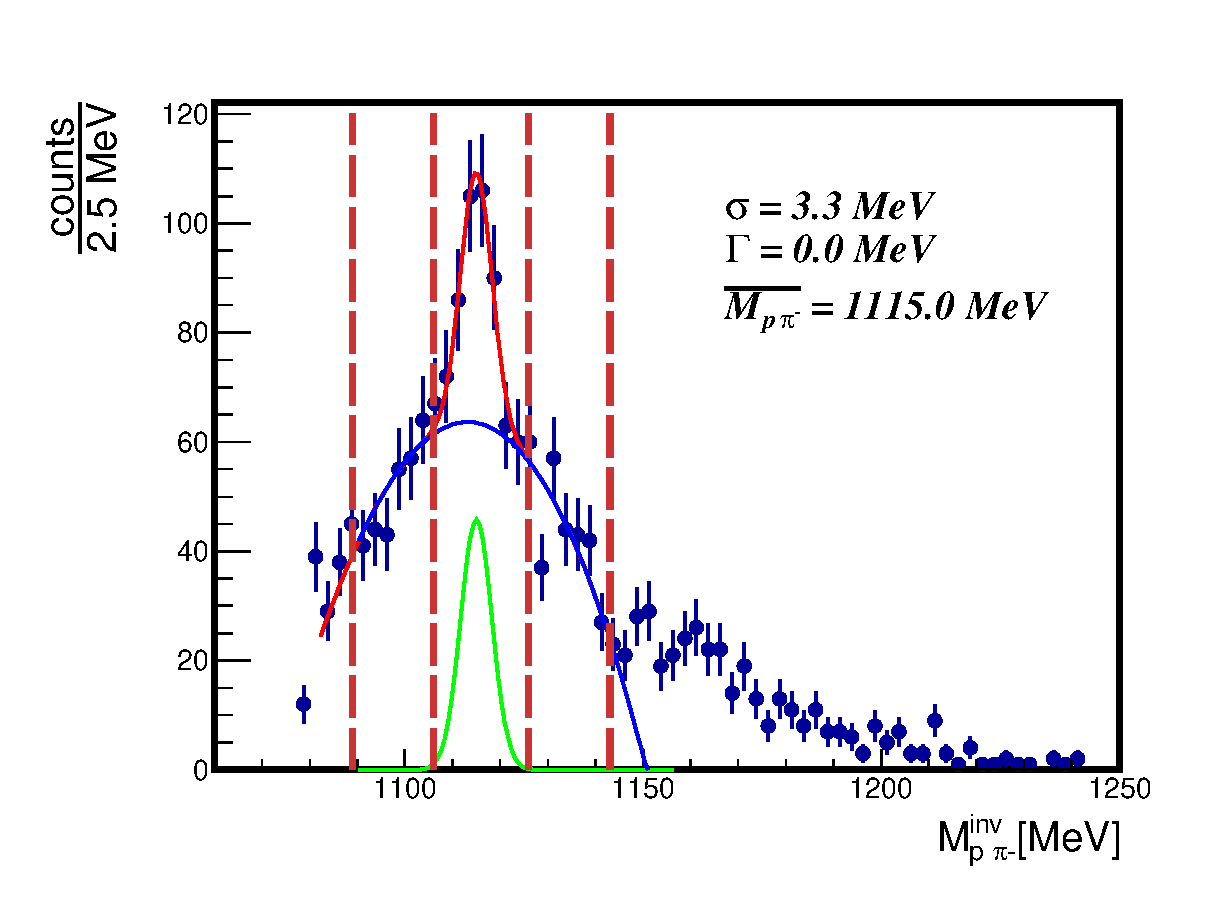
\includegraphics[width=0.7 \linewidth]{Chapter_analysis/L1116SB.eps}
  \caption{The $\Lz$ spectrum after a neural network analysis. The vertical lines denotes regions of a side-band analysis described in \ref{section:SB}. The data was fitted by a sum of 4-th order polynomial (blue line) and a Voigt function (green line. A very small value for $\Gamma$ paramiter is caused by the $\Lz$ long live-time. Obtained $\sigma$ value describe an aparatus energy resolution. }
  \label{fig:L1116SB}
\end{figure}


\section{The $\Lz \Kz $reconstruction}
\label{section:LzKz}
Because of a strangeness conservation low a $\Lz$ has to be produced with some anti-strange particle. The lightest candidate is a $\Kz$ meson, which decays in 69.2\% into $pip pim$ pair \cite{PDG}. For that reason a $\Lz \Kz$ signal is expected to be a significant part of the $\Lz \pip \pim$ final state.

After the $\Lz$ reconstruction two spectra were drown: a) a $\pip \pim$ invariant mass spectrum for events $1006<M^{inv}_{\p \pim}<1026$ and b) a $p pim$ invariant mass for $480 MeV<M^{inv}_{\pip \pim}<500 MeV$. The same analysis chain was used to analyzed all channels listed in \ref{tab:channels} which contains $\Lz$ and $\Kz$. In case of the reference channel the misssing mass cut was lowered to ???, what is a minimall missing mass expected for $pp \rightarrow p \Kz \Lz \pip$ reaction.

Using a procedure described in \ref{sec:normalization} the simulation was compared with experimental data (see \ref{fig:K0L0}). The simulation describes well a yeld of $\Kz$ and $\Lz$ produced in experiment, aldough it does not describe the background shape. This is mostly coused by lack of realable model for a double $\Dpp$ production. 

\begin{figure}[hb]
  \centering
  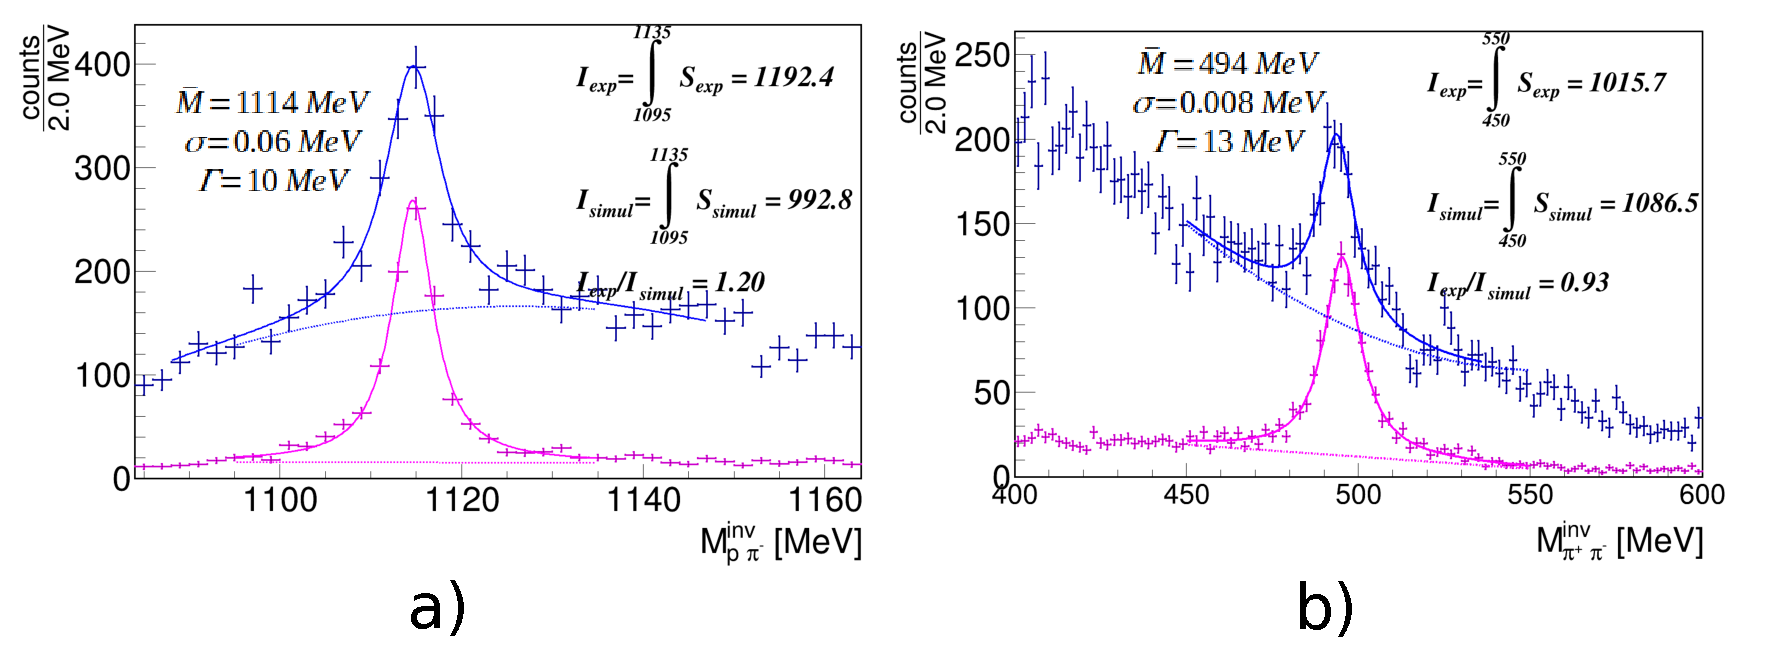
\includegraphics[width=0.9 \linewidth]{Chapter_analysis/K0L0.eps}
  \caption{The results for $\Lz \Kz$ asocieted production. Blue point reprezents experimental data, magenta a sum simulated channels. For both: the simulation and the experimental data a Voigt function was fited. Than, a total signal yeld between simulation and experiment was calculated.}
  \label{fig:K0L0}
\end{figure}

\section{Absolute normalization}
\label{sec:normalization}
An integrated luminosity for the pp experiment was calculated using a pp elastic scattering, it was
\begin{equation}
  L^{int}=3.13 \cdot 10^8 mb^{-1}.
\end{equation}
Thanks to a full scale simulation performed in HYDRA framework (for more details see chapter \ref{chapter:simulations}) it is posible to get a total detection eficiency for given reaction. The efficiency, together with known luminocity and a \cs allows for an expected count rate estimation, for any reaction.
\begin{equation}
  N^{\mathrm{expected}}_{pp\rightarrow X}=\frac{N_{\mathrm{detected}}}{N_{\mathrm{Simulated \; in \;} 4 \pi} \cdot 3} \cdot \sigma_{pp\rightarrow X} \cdot L.
\end{equation}
The factor 3 in denominator is connected with a trigger down-scaling. Due to limited read-out capabilities For a hadronic channels each 3th triggered event was seved on tapes. A list of the reactions used in following analysis are in \ref{tab:channels}. 
\begin{table}
    \centering
  \caption{List of the channels considered in following chapter. Numbers from 3 up to 10 indicates reactions containing $\p \pim \pip \pim$ in a final state. They are treated as a possible background channels. All values taken from \cite{hades_inclL_35}.}
  \label{tab:channels}
  \begin{tabular}{rll}
    \hline
    no. &Channel & $\sigma$ [$\mu \barn$]\\
    \hline
    \hline
    \multicolumn{3}{c}{3-body reactions} \\
    \hline
    1 & $\Lz \p \Kp$&$35.26 \pm 0.43 ^{+3.55}_{-2.83}$\\
    2 & $\Sz \p \Kp$&$16.5 \pm 20\%$\\
    3 & $\Lz \Dpp \Kz$&$29.45\pm 0.08 ^{+1.67}_{-1.46}\pm 2.06$\\
    4 & $\Sz \Dpp \Kz$&$9.26 \pm 0.05 ^{+1.41} _{0.31}\pm 0.65$\\
    5 & $\Sigma(1385)^+ \p \Kz$&$14.05 \pm 0.05 ^{+1.79}_{-2.14}\pm 1.00$\\
    6 & $\Dpp \Lss \Kz$&$5.0\pm 20\%$\\
    7 &$\Dpp \Ss \Kz$& $3.5 \pm 20\%$\\
    8 &$\Dp \Sigma(1358)^+ \Kz$&$2.3 \pm 20\%$\\
    \hline
    \multicolumn{3}{c}{4-body reactions} \\
    \hline
    9 &$\Lambda \p \pip \Kz $& $2.57 \pm 0.02 ^{+0.21}_{-1.98}\pm 0.18$\\
    10&$\Sz \p \pip \Kz$& $1.35 \pm 0.02 ^{+0.10}_{-1.35}\pm 0.09$\\
    \hline
  \end{tabular}
  
\end{table}


\section{The $\Ls$ Reconstruction}
\label{section:Ls}
The neural network analysis gives a data sample with good S/B ratio for $\Lz$ signal. However set of additional cuts has to be applayed ot extract a $\Ls$ signal from the data. Using the signal channel's simulation a set of hard cuts was optimalized: i) a distans between a secondary vertex (SV) and a primary vetex (PV) has to be larger than 5 mm, ii) an opening angle ($\mathrm{OA}_\Lz$) between a reconstructed $\Lz$ momentum direction and line connecting the primary and secondary vertexes has to be smaller than ?? . The cuts are ilustrated in fig. \ref{fig:Ls_cuts}. A $p \pim \pip \pim$ spectrum obtained after the hurt cuts contain both: a $\Ls$ singnal and background originated from background under a $\Lz$ peak. To remuve that contamination an additional steps were neccessery. One of them was a side-band analysis wich allowed to remove uncorelated combinatorial background from $\Ls$ spectrum.
\begin{figure}[hb]
  \centering
  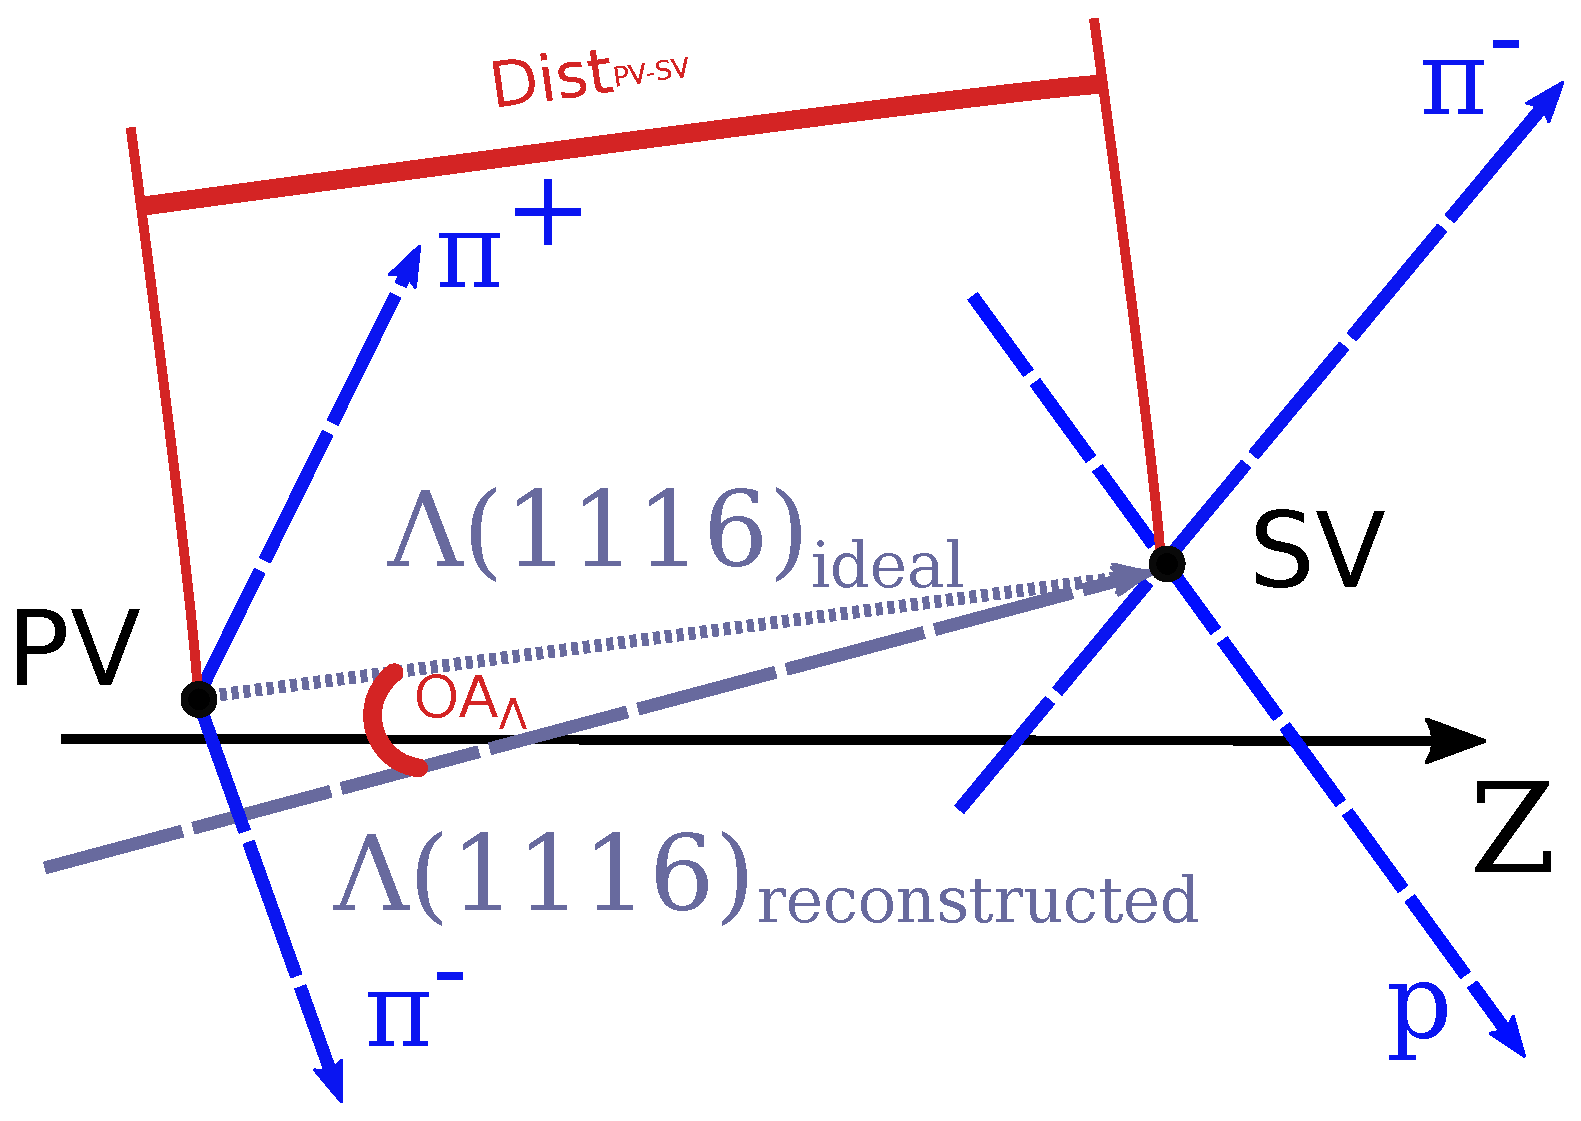
\includegraphics[width=0.7 \linewidth]{Chapter_analysis/geometria.eps}
  \caption{Cuts used for a $\Ls$ reconstruction. They were optimalized using simulation.}
  \label{fig:Ls_cuts}
\end{figure}



\subsection{Side-band analysis}
\label{section:SB}
A side-band analysis bases on assumption that a background kinematic changes slowlly through a spectrum. Thanks to this, kinematics of the background events from signal reagion can be well described by background outside the signal reagion. In case of described analysis the side-band methode was used to stimate an inpact of non-perfect $\Lz$ reconstruction for the $\Ls$ spectrum. The fig. \ref{fig:L1116SB} shows input for the side-band. The $p \pim \pip \pim$ spectra for the signal and SB region after all the cuts are shown in \ref{fig:Ls_SB}. The side-band describes wery welll both wings of the data distribution. A difference between signal and the side-band spectrum can be interpreted as $\p \pim \pip \pim$ signal associated with the $\Lz$ signal.
\begin{figure}[h]
  \centering
  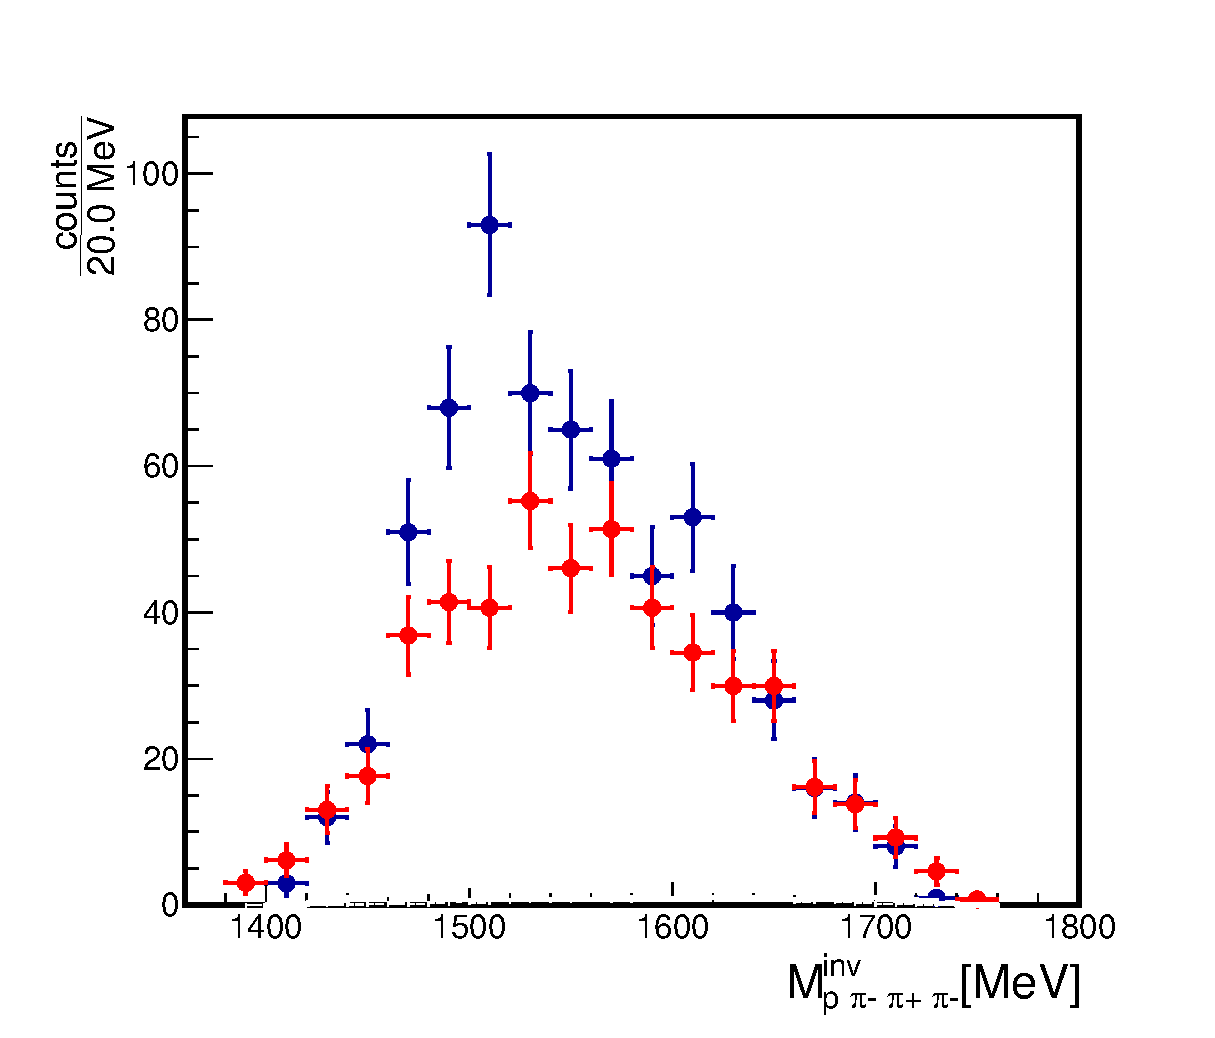
\includegraphics[width=0.7 \linewidth]{Chapter_analysis/L1520_sig_SB.eps}
  \caption{The $\Ls$ spectrum for events from signal reagion ($M_{\p \pim}^{inv}\in(1106,1126)$) -blue points, and from SB regions ($M_{\p \pim}^{inv}\in(1089,1106] \cup [1126,1143)$) - read points. Error bars shows a statistical uncertentity}
  \label{fig:Ls_SB}
\end{figure}

\subsection{Cross-section extraction differential analysis}
Despite the side-band spectrum describes a beckground shape very well, there is still some signal contamination in a mass region over 1540 MeV , see fig. ??. It may be caused by correlated combinatorial bacground, when a fake $\pip \pim$ pair is combinated with real $\Lz$ signal. The main source of di-pion pairs, a $\Kz$ decay, is supressed by a cut $M^{inv}_{\pip \pim}<410 MeV$. However there are reactions which allows for mixing pions from two different sources. Three of them were choosen as the most importat ones. They are presented in tab. \ref{tab:channels} with numbers 3-5. the final state for each of them contains $\Lz$ and two different sources of pions. An combination of a $\pim$ from a $\Kz$ decay and a $\pip$ from a $\Dpp$ or a $\mathrm{\Sigma^+}$ creates an coreleated combinatorial background.

An identyfication of the background channels allows to simmulate them and, together with a simulation of the signal channel estimate an inclusive \cs for
\begin{equation}
  \p\p \rightarrow \Ls \mathrm{X}
\end{equation}
reaction. The signal channel was simmulated according to exclusive cross section measured by HADES$\sigma_{\p\p\rightarrow \p \kp \Ls}
=6.5 \mathrm{\mu b}$ \cite{hades_L1520}. Next the simulated signal spectrum was scaled up to get the same area under a simulation and experimental histogram. Finally, according to the obtained scaling an inclusive \cs is equal $\sigma_{\p\p \rightarrow \Ls \mathrm{X}}=7.1\pm 1.5 \mathrm{\mu b}$. A uncertantity comes from a statistical error.

The total yeald of detected decays allows to cunduct a simple differential analysis. A transwers momentum ($p_t$) and rapidity ($\Upsilon$) was calculated for each reconstructed $\Ls$. Obtained spectra are presented in fig ???

\subsection{Analysis of a $\pip \pim$ spectrum}
In simulation model used for the \cs extraction pions were mitted accorgding to avaliable phase-space. However it is posible that pion production occures through a virtual $\rho$ meson. A possible $\rho$ contribution would manifest by a distortion of a $\pip \pim$ specrtum compared to direct production. An alternative simulation with the rho decay was alo prepared and both of them compared with experimental data. By naked eye an only-phase-space distribution describes data better. That was proven quantitatively making a linear combination of the two avaliable spectra
\begin{equation}
  sum=N \cdot M^{inv}_{\pip\pim_{\mathrm{w/o}} \rho} + (N-1) M^{inv}_{\pip\pim_\rho},
\end{equation}
where $N \in [0,1]$. An agreeement between data and simulation was tested by $\chi^2$ test. Its prooved that within avaliable errors the best data description is given by only-phase-space distribution of pions. 
\section{results from p Nb experiment}